Just like seismic motions contain a background of microseisms, atmospheric pressure also contains a backgroud od "microbaroms" that are radiated from ocean waves. However, this background is easily drowned in wind noise and is less visible than the microseism signal, and only in a narrow frequency window from 0.1 to 0.3~Hz. The first observations of microbaroms were made by \cite{Shuleikin1935} over the black Sea and \cite{Benioff&Gutemberg1939} on land. The first satisfactory theoretical explanation of microbarom generation for a homogeneous atmosphere was made by \cite{Brekhovskikh&al.1973} following the theories for microseisms. A recent extension of the theory to an ocean of finite depth was given by \cite{DeCarlo&al.2020} with a verification against measurements by \cite{DeCarlo&al.2021}, showing that it better fits observations than alternative or simplifiled theories.  This recent numerical modelling of microbaroms still contain a number of empirical adjustments, and here we will sketch how a more complete theory could be given, considering microbarom generation in the presence of atmospheric wave guides, instead of adding the effects of wave guides after the fact. Indeed, the main atmospheric wave guides that are followed by microbaroms go through the stratosphere or the mesosphere. As a result, microbaroms are of particular interested as a possible source for upper atmosphere tomography \citep{Donn&Rind1971,Smets&Evers2014} and the possiblity of detection of other signals in the 0.1 to 0.3~Hz band. More details about microbaroms can be found in \cite{DeCarlo2020}.

\section{Microbarom generation: piston effect}
The first qualitatively correct idea for the generation of microbaroms was formulated by \cite{Posmentier1967}, but it only strictly applies to vertically propagating acoustic waves. Here we use the generalization proposed by \cite{Ardhuin&Herbers2013}. 

We may consider the atmospheric motion to be irrotational, so that the equations of motion 
are identical in the atmosphere and in an unbounded ocean, with the only difference that 
 the atmospheric density is $\rho_a$ and the atmospheric sound speed is $\alpha_a$. We can thus use results from the previous chapter and first consider the solutions to the linearized acoustic equation eq. (\ref{eq:acoustic_linear}). 
 
The second-order velocity potential takes the form, 
\begin{equation}
 \phi_{2,a} \propto \exp[\ir(K_{x} x +K_{y} y + l_a z - \omega_s t)] \quad \mathrm{for} \quad z> 0,
\end{equation} 
with
\begin{equation}
 l_a= \sqrt{\frac{\omega_s^2}{\alpha_a^2} - K^2}.
\end{equation}

Because $\rho_w/\rho_a \simeq 1000$, the air motion has only a small $O(\rho_w/\rho_a)$ local 
influence on the water motion, so that the 
solutions derived earlier for the water motion remain valid in the presence of air. 
The air motion, with a velocity potential $\phi_a$ also obeying eq. (\ref{eq:acoustic_linear}) 
is fully determined from the 
water motion via the kinematic boundary conditions on the air and water-sides 
of the interface (\ref{surf_kine_Taylor}), 
\begin{equation}
     \frac{\partial \phi_a }{\partial z} - \frac{\partial \phi }{\partial z} \simeq 
\bnabla \left(\phi_a -\phi\right)\bcdot\bnabla \zeta  - \zeta \frac{\partial^2 \left(\phi_a -\phi\right) }{\partial^2 z} \quad{\mathrm{at}} \quad z=0. \label{surf_kine_Taylora}
\end{equation}
From the first order potential in the air \citep[e.g.][]{Waxler&Gilbert2006}
\begin{equation}
     \phi_{1} = \sum_{\kb,s} \ir s \frac{g}{\sigma}   Z_{1,\kb}^{s}  \er^{-kz} \er^{\ir\left(\kb \bcdot{\mathbf x} - s \sigma\right)} 
\end{equation}
we obtain the second order potential, 
\begin{equation}
      \frac{\partial \phi_{2,a} }{\partial z} =\frac{\partial \phi_2}{\partial z} 
                    + \sum_{\kb,s,\kpb,s'}  D_{za} \left(\kb,s,\kpb,s',z \right) Z_{1,\kb}^{s} Z_{1,\kpb}^{s'} 
\mathrm{e}^{\mathrm{i}
    \Theta(\kb,\kpb,s,s')}\nonumber \\ \label{P2a}
\end{equation}
and a new coupling coefficient
\begin{eqnarray}
D_{za} \left(\kb,s,\kpb,s',z\right)   = -\frac{2 \ir s g}{\sigma} \left(k k' + \kb \bcdot \kpb\right). \nonumber \\ \label{Dza}
\end{eqnarray}

We note that for $\kpb = -\kb$, $D_{za}=0$, so that the long-wavelength motion with $K \ll k$ simplifies to 
\begin{equation}
     \frac{\partial \phi_{2a} }{\partial z} \simeq  \frac{\partial \phi_2 }{\partial z}   \quad{\mathrm{at}} \quad z=0. \label{surf_kine_Tayloratm}
\end{equation}
consistent with the result given by \cite{Posmentier1967} for the interaction of monochromatic wave trains, 
and in disagreement with a factor 8 correction proposed by \cite{Arendt&Fritts2000}. This equation basically says that, at the surface, the vertical velocity in the air is equal to the vertical velocity in the water. In other words the surface is like a piston that transmits water motion to the air. 

It all looks good except that, the vertical derivatives introduce the vertical wavenumbers in the air and in the water, so that the power spectrum of the atmospheric pressure is, 
\begin{equation}
F_{p2,ap}(\Kb,f_s)= \frac{\rho_a^2 \left|l^2\right|}{\rho_w^2 l_a^2 } 
F_{p2,\mathrm{surf}}(\Kb ,f_s)
\end{equation}
Which goes to infinity when $l_a$ goes to zero, i.e. for horizontal propagation in the atmosphere that corresponds to a propagation angle in the water close to 12 degrees from the vertical. Clearly, some of our hypotheses do not apply as the atmospheric propagation angle goes to the horizontal. This problem was solved by \cite{Brekhovskikh&al.1973}, and it is explained in details by \cite{DeCarlo2020}. In fact the expression above here is good down to angles of 1$^\circ$ from the horizontal. In general we find 
\begin{equation}
F_{p2,ap}(\Kb,f_s)= \frac{\rho_a^2 R_a^2}{\rho_w^2 } 
F_{p2,\mathrm{surf}}(\Kb ,f_s),
\end{equation}
with $R_a$ shown in Fig. \ref{fig:rad_deep}.
The ocean surface is thus a very strange piston that radiates most of the acoustic energy at angles close to the horizontal.
%%%%%%%%%%%%%%%%%%%%%%%%%%%
\begin{figure}[htb]
\centering
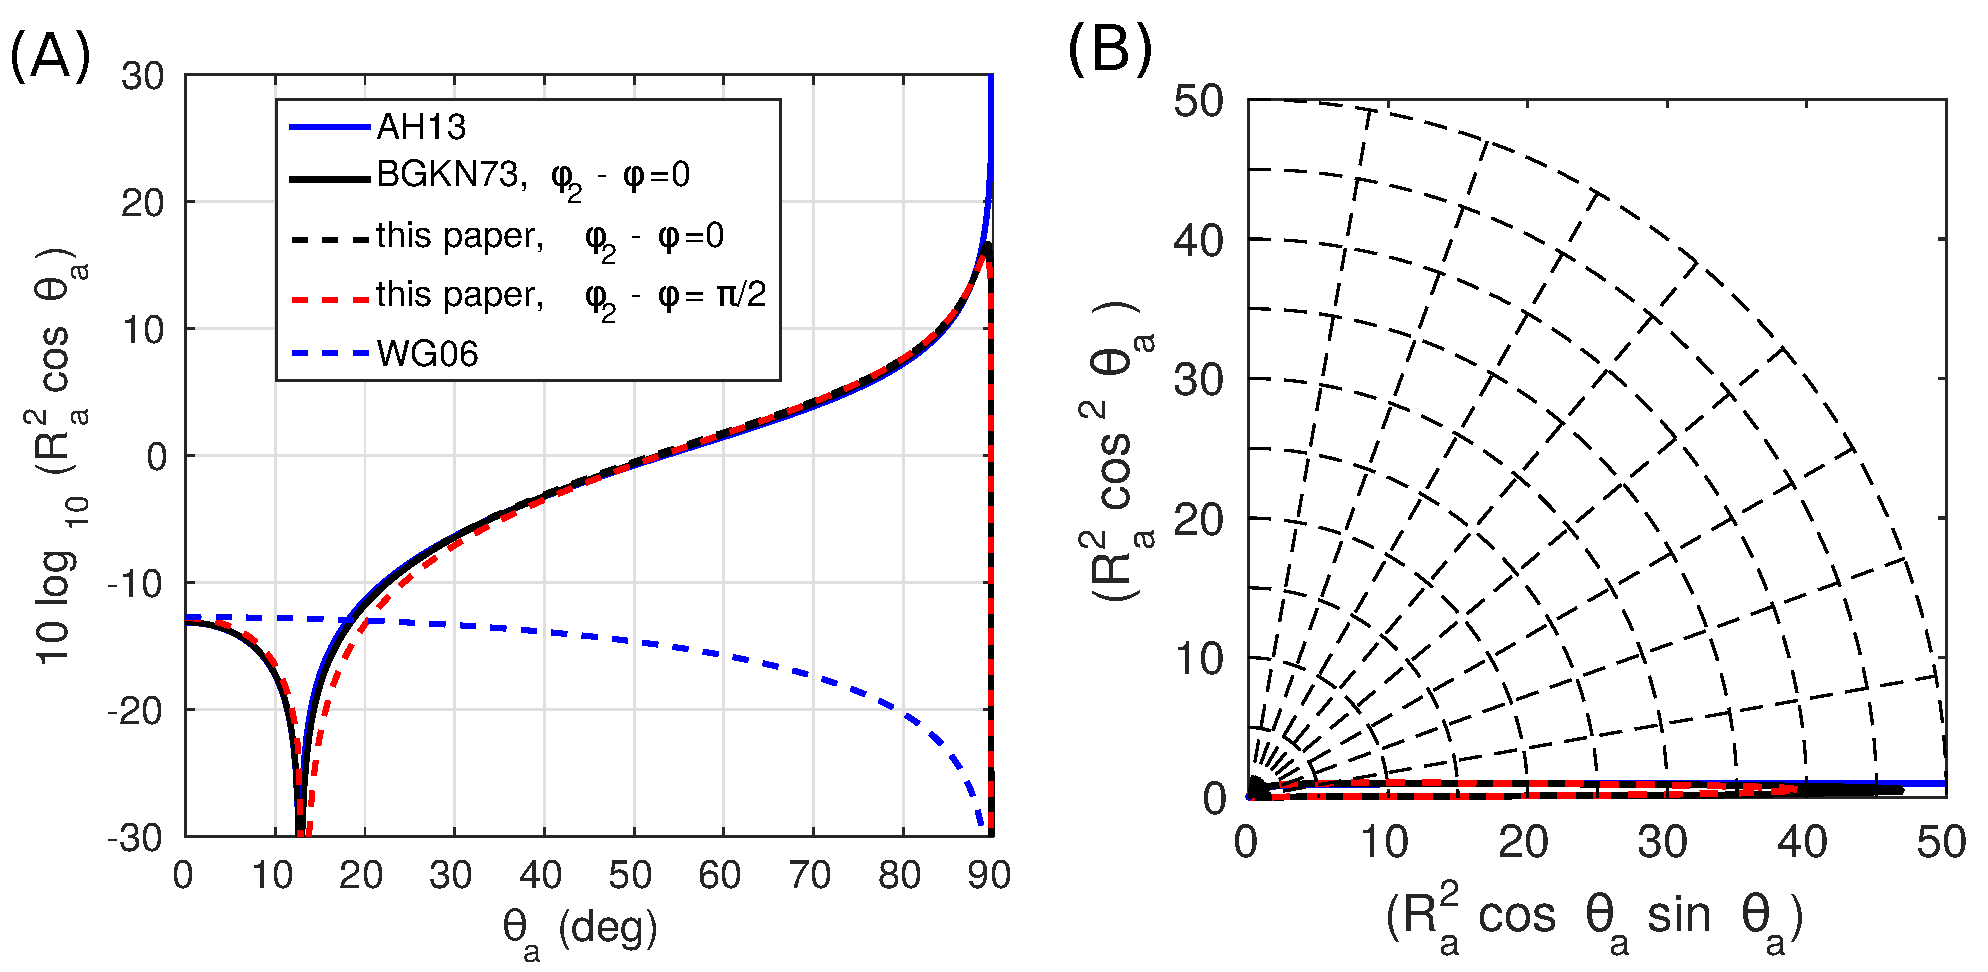
\includegraphics[width=0.8\linewidth]{FIGURES/radiation_deep.pdf}
\caption{Radiation patterns for an ocean wave period of 10~s, given by the different theories without ocean bottom, in cartesian (A), and polar (B) representation, as a function of the acoustic propagation elevation angle $\theta_a$ (measured from the vertical). Note that when the radiated power is considered, these patterns must be multiplied by $\sin \theta_a$ before integration over $\theta_a$. Reproduced from De Carlo et al. (2020). %, as given by eq. (\ref{eq:Power_thetaa}).
  }
\label{fig:rad_deep}
\end{figure}
%%%%%%%%%%%%%%%%%%%%%%%%%%

For a quantitatively correct solution we have to keep all the terms in the equation, including the feedback of the atmospheric pressure on the ocean.
For now, please go to chapter 3 of \cite{DeCarlo2020}. You may find more details here in the next version. In particular I may be brave enough to give you the microbarom source for a 2-layer or $n$-layer atmosphere to show how wave guides can be introduced in the theory without ad hoc handwaving. 



